\subsection{Impact of Cross Traffic}\label{s:robust:cross}

\begin{figure*}
\begin{centering}
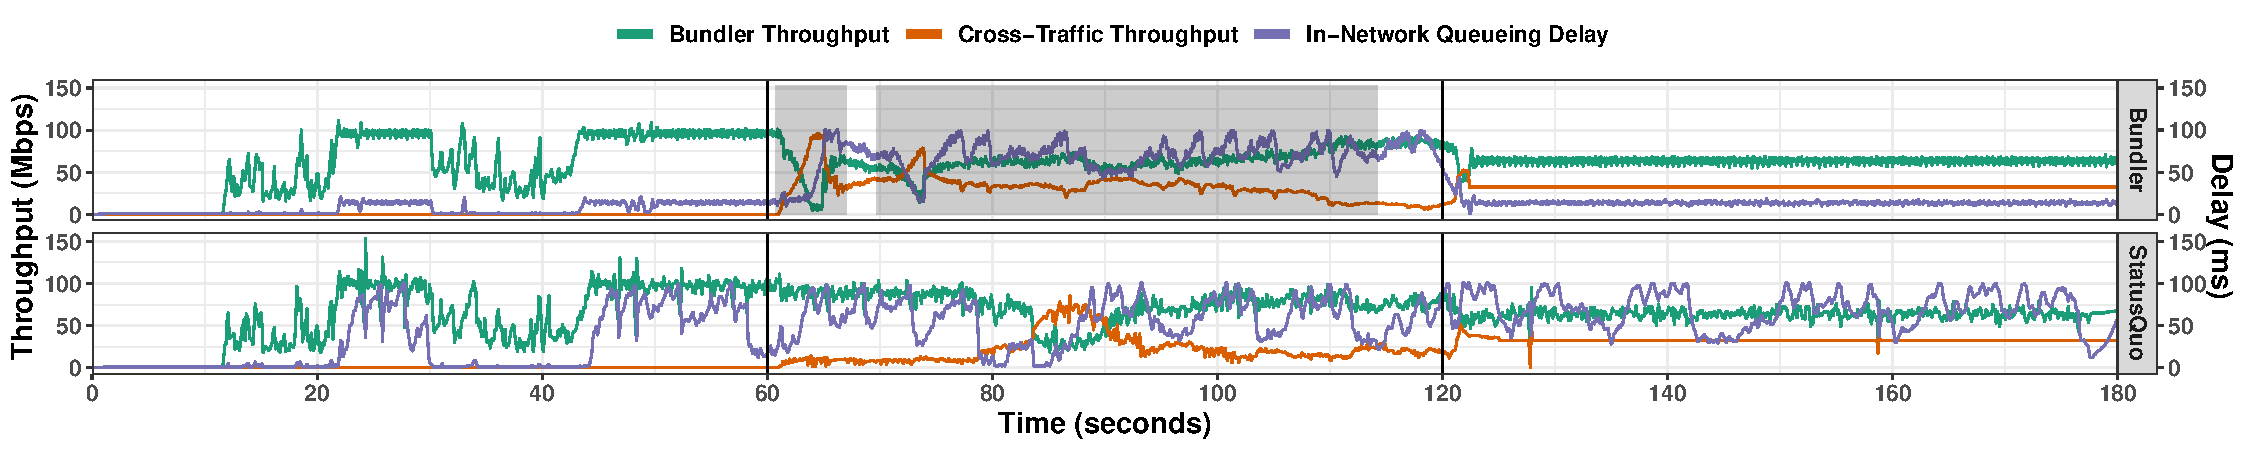
\includegraphics[width=\textwidth]{big_exp/timeseries}
\end{centering}
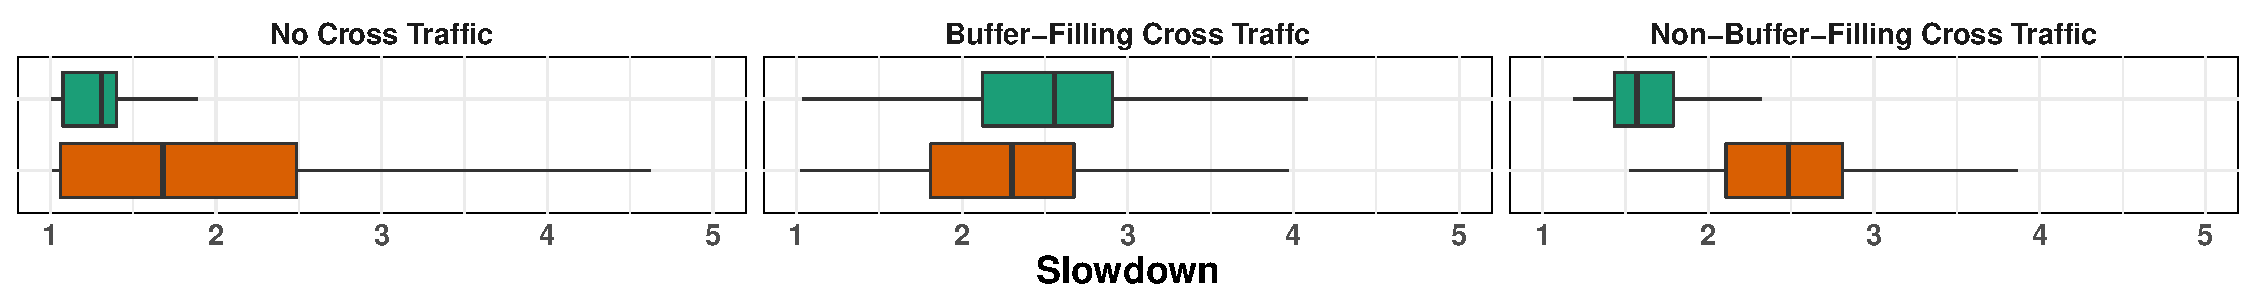
\includegraphics[width=0.95\textwidth]{big_exp/fcts}
\caption{\name's scheduling ability depends on the characteristics of the cross traffic over time. In this experiment, there are 3 periods: from 0 to 60 sec., there is no competing traffic, from 60 to 120 sec. there is buffer-filling cross traffic, and from 120 to 180 sec. there is non-buffer-filling cross traffic. The box-plots below each period show the distribution of short flow FCTs during that time. During the period with buffer-filling cross traffic, \name detects its presence and competes fairly. The shaded region indicates time \name spent in buffer-filling cross-traffic mode (\Sec{s:buffer-filling}).}\label{fig:eval:bigexp}
\end{figure*}

Can \name successfully revert to status-quo performance in the presence of buffer-filling cross traffic, then resume providing benefits once that cross traffic leaves?
In Figure~\ref{fig:eval:bigexp}, we show this scenario.
At first, the link is occupied only by \name's traffic, similar to the setup described in \S\ref{s:eval:setup}.
\radhika{do we have a backlog flow in the bundle here? If yes, mention it. If not, delete this comment.}
At time $t=60$sec, a buffer-filling cross traffic flow arrives.
\name detects its presence (indicated by the gray shading) and reverts to performance that is slightly worse than Status Quo. It is slightly worse because of the small queue that \name continues to maintain at its \inbox for active probing to detect the cross-traffic's departure, as described in \S\ref{s:queue-ctl}.\footnote{We believe the benefits provided by \name in the more common regime with no competing buffer filling cross traffic are substantial enough to allow for this slight degradation in these specific scenarios.}  \radhika{edited last two sentences. pls check.}
At time $t=120$sec, the buffer-filling flow stops and non-buffer-filling traffic starts, generated from the same distribution as \name as described in \S\ref{s:eval:setup}.
\name correctly detects that it is safe to resume delay-control, and continues providing scheduling benefits.
\radhika{In the graph, rewrite `Queueing Delay' as `In-network Queueing Delay'.} 
For the remainder of this subsection, we present three micro-benchmarks which dig deeper into the latter two scenarios, where cross traffic can affect \name's performance. 
We present results with both Nimbus and Copa being used as the congestion control algorithm at the \inbox.

\begin{figure}
    \centering
\begin{knitrout}
\definecolor{shadecolor}{rgb}{0.969, 0.969, 0.969}\color{fgcolor}
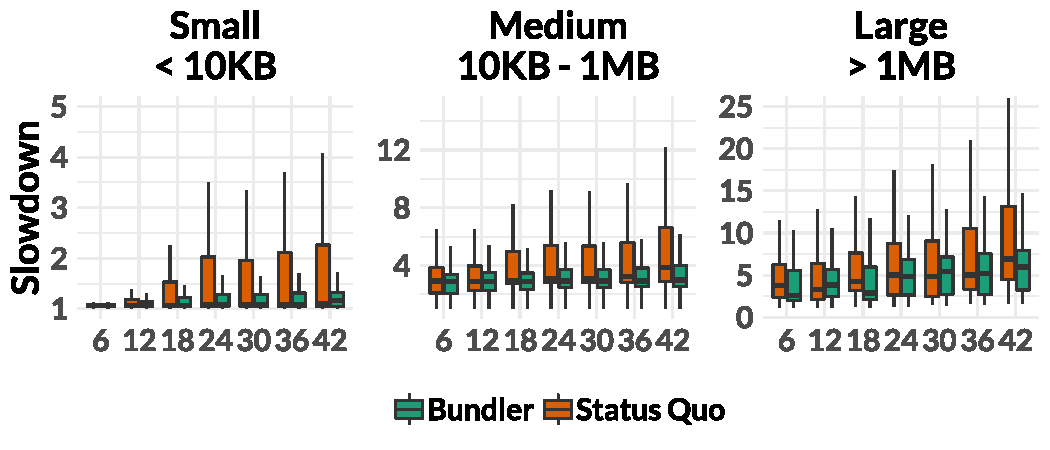
\includegraphics[width=\maxwidth]{figure/robust_cr-inelastic-1} 

\end{knitrout}
    \caption{Against cross traffic comprising of short lived flows. \name offers 48Mbps of load to the bottleneck queue. The cross traffic's offered load increases along the x-axis, while \name{}'s offered load remains fixed.}
    \label{fig:robust:cr-inelastic}
\end{figure}

\paragrapha{Short-lived flows} We first consider the case where the cross traffic comprises of short-lived flows up to a few MBs.
We keep \name's offered load (comprising of web requests described in \S\ref{s:eval:setup}) constant, but vary the cross traffic's offered load.
Figure~\ref{fig:robust:cr-inelastic} shows that \name continues to provide benefits for this case, since maintaining low in-network queues is still possible in the presence of such flows.

\begin{figure}
    \centering
    \begin{subfigure}[b]{0.5\textwidth}
\begin{knitrout}
\definecolor{shadecolor}{rgb}{0.969, 0.969, 0.969}\color{fgcolor}
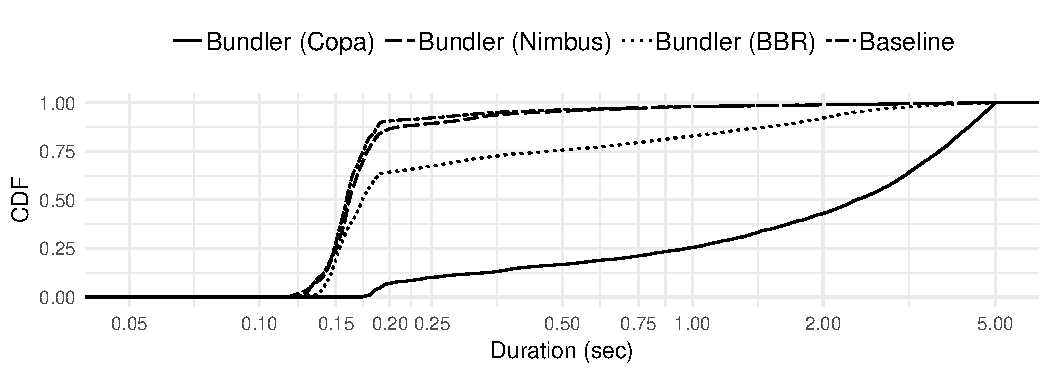
\includegraphics[width=\maxwidth]{figure/robust:cr-elastic:a-1} 

\end{knitrout}
    \caption{Congestion controllers from \S\ref{s:eval}.}\label{fig:robust:cr-elastic:a}
    \end{subfigure}
    \begin{subfigure}[b]{0.5\textwidth}
\begin{knitrout}
\definecolor{shadecolor}{rgb}{0.969, 0.969, 0.969}\color{fgcolor}
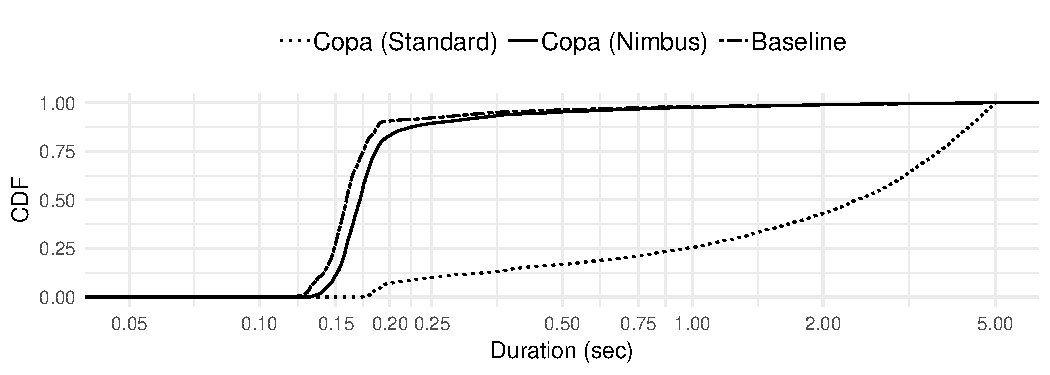
\includegraphics[width=\maxwidth]{figure/robust:cr-elastic:b-1} 

\end{knitrout}
    \caption{Alternate configuration -- Copa uses Nimbus's elasticity detector.}\label{fig:robust:cr-elastic:b}
    \end{subfigure}

    \caption{Elastic cross traffic.}
    \label{fig:robust:cr-elastic}
\end{figure}


\newcommand{\bigexpBundlerElasticSlowdown}{2.6251566\%\xspace}
\newcommand{\bigexpNoBundlerElasticSlowdown}{2.3453956\%\xspace}
\newcommand{\bigexpElasticSlowdownWorseness}{12\%\xspace}

\paragrapha{Buffer-filling flows} Competition from persistent backlogged flows (recall from \S\ref{s:deploy} that this condition is rare) that fill the bottleneck link's buffer is the worst-case scenario for \name.
As described in \S\ref{s:queue-ctl}, \name's congestion controller must push packets into the bottleneck queue to compete fairly, and thus it cannot retain packets at the \inbox for scheduling. 
Furthermore, recall that \name maintains a $10$ms queue at the \inbox in this case. Thus, we expect component flows to experience RTT unfairness.
We indeed see this in Figure~\ref{fig:robust:cr-elastic}, as we vary the number of competing Cubic cross-traffic flows.
As expected, the component flows, on aggregate, experience \bundlerElasticTputWorseness less throughput on average.
Note that FCTs may not increase as much; in Figure~\ref{fig:eval:bigexp}, during the elastic cross traffic period the median short flow FCT is
\bigexpElasticSlowdownWorseness higher.

\begin{figure}
    \centering
\begin{knitrout}
\definecolor{shadecolor}{rgb}{0.969, 0.969, 0.969}\color{fgcolor}
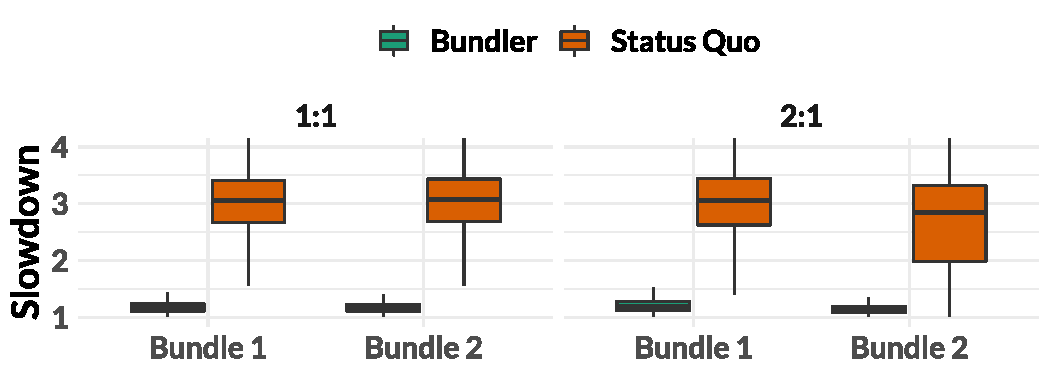
\includegraphics[width=\maxwidth]{figure/robust_twobundler-1} 

\end{knitrout}
    \caption{Competing traffic bundles. In both cases, the aggregate offered load is 84Mbps, as in Figure~\ref{fig:eval:best}. For "1:1", we evenly split the offered load between the two Bundles; for "2:1", one bundle has twice the offered load of the other. In both cases, each bundle observes improved median FCT compared to its performance in the baseline scenario.}
    \label{fig:robust:twobundler}
\end{figure}

\paragrapha{Competing Bundles} Last, we evaluate the case where flows from multiple bundles compete with one another. 
In Figure~\ref{fig:robust:twobundler}, we show the performance with two bundles of traffic competing with one another at the same bottleneck link. 
Both bundles comprise of web requests along with a backlogged Cubic flow. 
Even in the presence of this buffer-filling cross traffic, both bundles maintain low queueing in the network and successfully control the queues at the \inbox.
Thus, \name provides benefits for both bundles, even when the amount of traffic in each bundle is different.  

\subsection{Impact of Congestion Control}\label{s:eval:cc}

We now evaluate the impact of a different congestion control algorithm running at the \inbox and at the endhosts.

\begin{figure}
    \centering
\begin{knitrout}
\definecolor{shadecolor}{rgb}{0.969, 0.969, 0.969}\color{fgcolor}
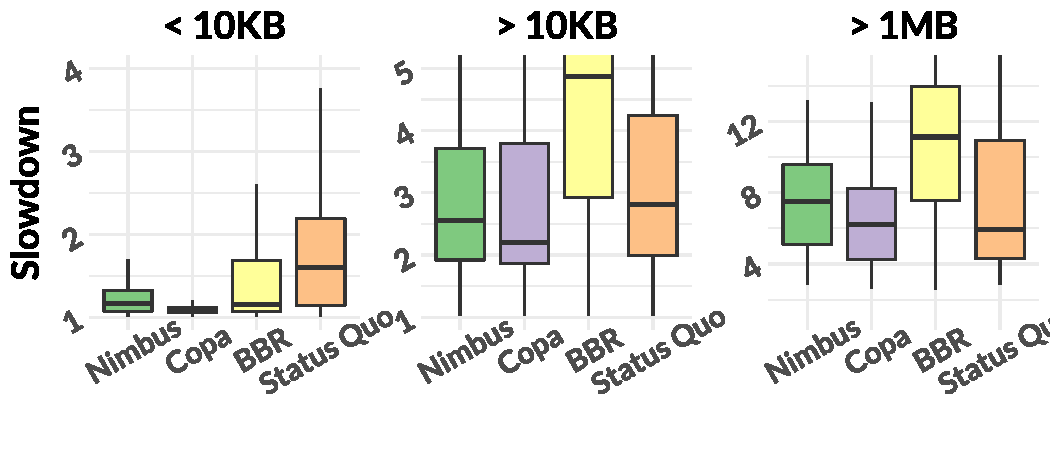
\includegraphics[width=\maxwidth]{figure/eval:cc-1} 

\end{knitrout}
    \caption{Choosing a congestion control algorithm at \name remains important, just as it is at the end-host. Note the different y-axis scales for each group of request sizes.}
    \label{fig:eval:cc}
\end{figure}
\newcommand{\ccCopaMedian}{}
\newcommand{\ccNimbusMedian}{}
\newcommand{\ccBBRMedian}{}
\newcommand{\ccBaselineMedian}{}


\Para{\capinbox congestion control} So far we have evaluated \name by running Copa~\cite{copa} at the \inbox.  
Figure~\ref{fig:eval:cc} shows \name's performance with other congestion control algorithms (namely, Nimbus~\cite{nimbus} and BBR~\cite{bbr}), and using SFQ scheduling. 
We find that using Nimbus provides similar benefits over \baseline as Copa. 
BBR, on the other hand, performs slightly worse than \baseline. 
This is because it pushes packets into the network more aggressively than the other schemes, resulting in a bigger in-network queue.
This, combined with the queue built at the \name, results in the endhosts experiencing higher queueing delays than \baseline. This shows that the choice of congestion control algorithm, and its ability to maintain small queues in the network, plays an important role. 

\begin{figure}
    \centering
\begin{knitrout}
\definecolor{shadecolor}{rgb}{0.969, 0.969, 0.969}\color{fgcolor}

\includegraphics[width=\maxwidth]{figure/eval_e2e-1} 

\end{knitrout}
    \caption{\name still provides benefits when the endhosts use different congestion control algorithms.}
    \label{fig:eval:traffic}
\end{figure}

\Para{Endhost congestion control} 
We used Cubic congestion control at the endhosts for our experiments so far. When we configure endhosts to use BBR (as implemented in Linux $4.13$), \name's benefits remain: in Figure~\ref{fig:eval:traffic}, \name achieves 58\% lower FCTs in the median compared to the updated \baseline where the endhosts use BBR. 
This is primarily because in the \baseline using BBR causes endhosts to achieve 66\% worse median slowdown ($1.62$ with Cubic to $2.68$ with BBR); \name's slowdown is only 5\% worse when endhosts use BBR ($1.08$ with Cubic to $1.14$ with BBR). 
This shows that \name is compatible with multiple endhost congestion control algorithms.
